\scanpage{215}
\mspage{214}
(Résulte de la conjonction des conj. de
Hodge et de Tate \inserted{\figure{\begin{tikzpicture}\node[draw,ellipse] {sur corps finis};\end{tikzpicture}}}, au moins si $X$
\uline{normal}). \uline{\uuline{\unsure{Caractériser} \deleted{de} l'image}} ??

\margin{\figure{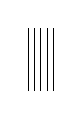
\begin{tikzpicture}\foreach \x in {0,.08,.16,.24,.32}{\draw (\x,0)--(\x,.8);}\end{tikzpicture}}}
Même conclusion si $X$ défini sur $h\subset C$, $h$ alg.
clos, p.ex. $h=\overline{\mathbb Q}$.

\uline{Analyser l'exemple de Serre de} $\pi_1$ \uline{non
isomorphes}

[\uline{Cas corps de base} $\mathbb R$ : tout pt \deleted{réel}\inserted{géom. $a$} définit
une $\xi_a\in T_\alpha(\mathbb Z)$. Tous les $\xi_a$ sont isom.
\unsure{pour} \inserted{si}\deleted{\unsure{e}} $X$ est \deleted{géom. connexe}\inserted{irred (pas néc. géom irred)}.
\deleted{Il peut y \unsure{en avoir} deux non isom.}
Si $a$ est un pt réel, alors $\xi_a$ admet
un autom $\operatorname{frob}_\infty$ d'ordre $2$, qui
avec la comp. conn. de $G(X,\xi)$ engendre
$G(X,\xi)$. Le foncteur
\[
M\longmapsto\bigl(\xi(M),+\text{structure de Hodge}
+\text{réellification définie par }\operatorname{frob}_\infty\bigr)
\]
est pleinement fidèle.]

\margin{\diagram{\begin{tikzcd}[row sep=small,column sep=small]
& X\arrow[dl,no head]\arrow[dd,no head]\\
C\arrow[dr,no head]&\\
& R
\end{tikzcd}}}

\margin{\figure{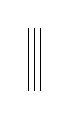
\begin{tikzpicture}\foreach \x in {0,.08,.16}{\draw (\x,0)--(\x,.8);}\end{tikzpicture}}}
\uline{Pb} étudier comment varie la structure
de Hodge sur un pt \inserted{complexe} variable, \uline{en fonction de
la donnée définie} en le pt $a_0$.
